\documentclass[12pt]{article}

% ---------- Formatting per report guideline ----------
\usepackage[margin=1in]{geometry}
\usepackage{mathptmx}        % Times New Roman equivalent for LaTeX
\usepackage{setspace}
\setstretch{1.15}
\usepackage[justification=justified]{caption}
\usepackage{ragged2e}
\usepackage{graphicx}
\usepackage{booktabs}
\usepackage{array}
\usepackage{enumitem}
\usepackage{amsmath}
\usepackage[hidelinks]{hyperref}

\title{\vspace{-1.5em}Inventory Analytics for EV Spare Parts}
\author{}
\date{}

\begin{document}
\maketitle
\vspace{-2.5em}

\begin{center}
\textbf{Group members:} [Name 1], [Name 2], [Name 3] \\
\textit{Fill in your team's names here before submitting.}
\end{center}

\vspace{0.5em}

% ============================================================
\section*{1. Problem Statement and Objective}

A regional EV service company operates a central spare-parts warehouse supplying several
service centers. Demand for spare parts is uncertain: some parts are ordered routinely, while
others are expensive and rarely demanded but critical when needed. Poor inventory planning
creates two opposing costs -- excess stock ties up capital and incurs holding cost, while
insufficient stock causes stockouts, delayed repairs, and lost service revenue.

The warehouse manager wants to move beyond simply forecasting demand accurately, toward
understanding the \emph{operational cost} of forecasting errors. This project analyzes 78
weeks of historical demand and inventory data across 24 spare parts, compares several
forecasting methods using both statistical error and business cost, and produces concrete
reorder recommendations.

\textbf{Central question:} \emph{Can a forecasting method with low statistical error still
create high inventory cost?}

\textbf{Scope:} the analysis covers data validation, exploratory analysis of demand and
inventory performance, four forecasting methods evaluated via walk-forward validation, a dual
(error vs.\ cost) evaluation, and a reorder-point recommendation system exported as a CSV
deliverable.

% ============================================================
\section*{2. Data and Assumptions}

Three weekly tables were used: \texttt{parts.csv} (24 parts; cost, price, lead time, holding
and stockout cost rates), \texttt{demand.csv} (units requested per part per week), and
\texttt{inventory.csv} (stock on hand and replenishment per part per week, before demand is
fulfilled). All three were validated to contain no missing values, no duplicate keys, no date
gaps, and no negative values before any further analysis.

After merging demand and inventory on \texttt{(week\_start, part\_id)}, five variables were
derived exactly as specified:
\begin{itemize}[nosep]
  \item \texttt{available\_inventory = stock\_on\_hand + replenishment}
  \item \texttt{units\_fulfilled = min(available\_inventory, units\_demanded)}
  \item \texttt{unmet\_demand = max(units\_demanded - available\_inventory, 0)}
  \item \texttt{ending\_stock = max(available\_inventory - units\_demanded, 0)}
  \item \texttt{stockout = 1} if \texttt{unmet\_demand > 0}, else \texttt{0}
\end{itemize}
Reconciliation (demand = fulfilled + unmet) and the week-to-week stock-chaining property were
both verified across the full dataset.

\textbf{Key assumptions, stated explicitly:}
\begin{itemize}[nosep]
  \item Forecasts and order quantities are rounded to integer units before any inventory
  calculation.
  \item A time-based 75/25 train/test split (58/20 weeks) is used, never shuffled.
  \item MAPE excludes zero-demand weeks to avoid division by zero.
  \item Cost model: overage (forecast $>$ actual) is costed at
  \texttt{holding\_cost\_per\_unit\_week}; underage (forecast $<$ actual) is costed at
  \texttt{stockout\_cost\_per\_unit}. Each week's forecast is treated as the stocking
  decision that would have been made.
  \item Safety stock uses a fixed 95\% service level ($z = 1.65$) applied uniformly; a
  per-part newsvendor critical ratio was tested first but rejected because
  \texttt{stockout\_cost\_per\_unit} exceeds \texttt{holding\_cost\_per\_unit\_week} by 1--2
  orders of magnitude for every part, causing the ratio to saturate near 1.0 and lose any
  differentiating power.
  \item A weekly review cycle is assumed, so recommended order quantity brings stock up to
  the reorder point with no additional review-period buffer.
\end{itemize}

% ============================================================
\section*{3. Methodology: Algorithmic Workflow}

The analysis proceeds through six phases. The two most decision-heavy components --
walk-forward forecasting and reorder classification -- are given in pseudocode below; the
remaining phases (data audit, merge, EDA, cost aggregation) are straightforward
groupby/aggregate operations over the merged weekly table.

\begin{quote}
\small\ttfamily\noindent
\textbf{Algorithm 1: Walk-forward forecast evaluation}\\[0.3em]
methods = \{naive, moving\_average, exp\_smoothing, holt\}\\
\textbf{for} each part $p$ in 24 parts:\\
\hspace*{1.5em}series = sorted weekly demand for $p$\\
\hspace*{1.5em}\textbf{for} each test week $t$ (20 weeks, chronological):\\
\hspace*{3em}history = series[week $<$ $t$] \quad\% never includes $t$ or later\\
\hspace*{3em}actual = series[$t$]\\
\hspace*{3em}\textbf{for} each method $m$ in methods:\\
\hspace*{4.5em}forecast = round(clip($m$(history), 0, $\infty$))\\
\hspace*{4.5em}record ($p$, $t$, $m$, forecast, actual)\\
\textbf{return} long table of (part, week, method, forecast, actual)
\end{quote}

\begin{quote}
\footnotesize\ttfamily\noindent
\textbf{Algorithm 2: Reorder classification} (checked in order; first match wins)\\[0.3em]
\textbf{function} classify(part):\\
\hspace*{1.5em}\textbf{if} current\_stock $<$ reorder\_point:\\
\hspace*{3em}\textbf{return} "Needs immediate replenishment"\\
\hspace*{1.5em}\textbf{else if} stockout\_rate $>$ 0.05:\\
\hspace*{3em}\textbf{return} "High stockout risk"\\
\hspace*{1.5em}\textbf{else if} unit\_cost $>$ median\_cost \textbf{and} mean\_demand $<$ median\_demand:\\
\hspace*{3em}\textbf{return} "Expensive low-demand -- do not overstock"\\
\hspace*{1.5em}\textbf{else if} current\_stock $>$ 2 $\times$ reorder\_point:\\
\hspace*{3em}\textbf{return} "Excessive inventory"\\
\hspace*{1.5em}\textbf{else}:\\
\hspace*{3em}\textbf{return} "Adequate -- no action needed"
\end{quote}

\textbf{Demand pattern classification} used the Syntetos--Boylan method (ADI and CV$^2$)
rather than an arbitrary zero-demand threshold: ADI $= n / n_0$ (weeks over nonzero-demand
weeks) and CV$^2 = (s_0/\bar{x}_0)^2$ over nonzero weeks. All 24 parts classified as
\emph{Smooth} (ADI $\approx 1.0$, CV$^2 < 0.49$), ruling out Croston's method. Holt's method
(trend, no seasonal component -- 78 weeks is insufficient for a full seasonal cycle) was kept
in the comparison regardless, letting the cost evaluation decide its value empirically.

\textbf{Safety stock and reorder point:}
\[
\text{safety\_stock} = \lceil z \cdot \sigma_{\text{demand}} \cdot \sqrt{L} \rceil, \qquad
\text{reorder\_point} = \lceil \hat{d} \cdot L + \text{safety\_stock} \rceil
\]
where $L$ is lead time in weeks, $\sigma_{\text{demand}}$ is each part's weekly demand
standard deviation, and $\hat{d}$ is the forecasted weekly demand from its cost-cheapest
method.

% ============================================================
\section*{4. Findings and Managerial Insights}

\textbf{Error vs.\ cost, in aggregate:} averaged across all 24 parts, Holt's method was both
the most accurate (MAE 3.17, MAPE 33.7\%) and the cheapest (average total cost \$5{,}714),
ahead of exponential smoothing, moving average, and naive (worst on every metric).

\textbf{The disagreement -- the central result:} at the level of individual parts, this
agreement breaks down. On 11 of 24 parts, the most statistically accurate method was
\emph{not} the cheapest one -- choosing accuracy over cost on those parts costs \textbf{35.8\%
more on average}, peaking at \textbf{152.9\% more} on part P023 (Figure~\ref{fig:disagreement}).
A robustness check using RMSE instead of MAE to define "most accurate" gives 9 of 24 parts
disagreeing (7 in common with the MAE-based set) -- a similarly-sized effect, not an artifact
of one specific metric.

\begin{figure}[h]
  \centering
  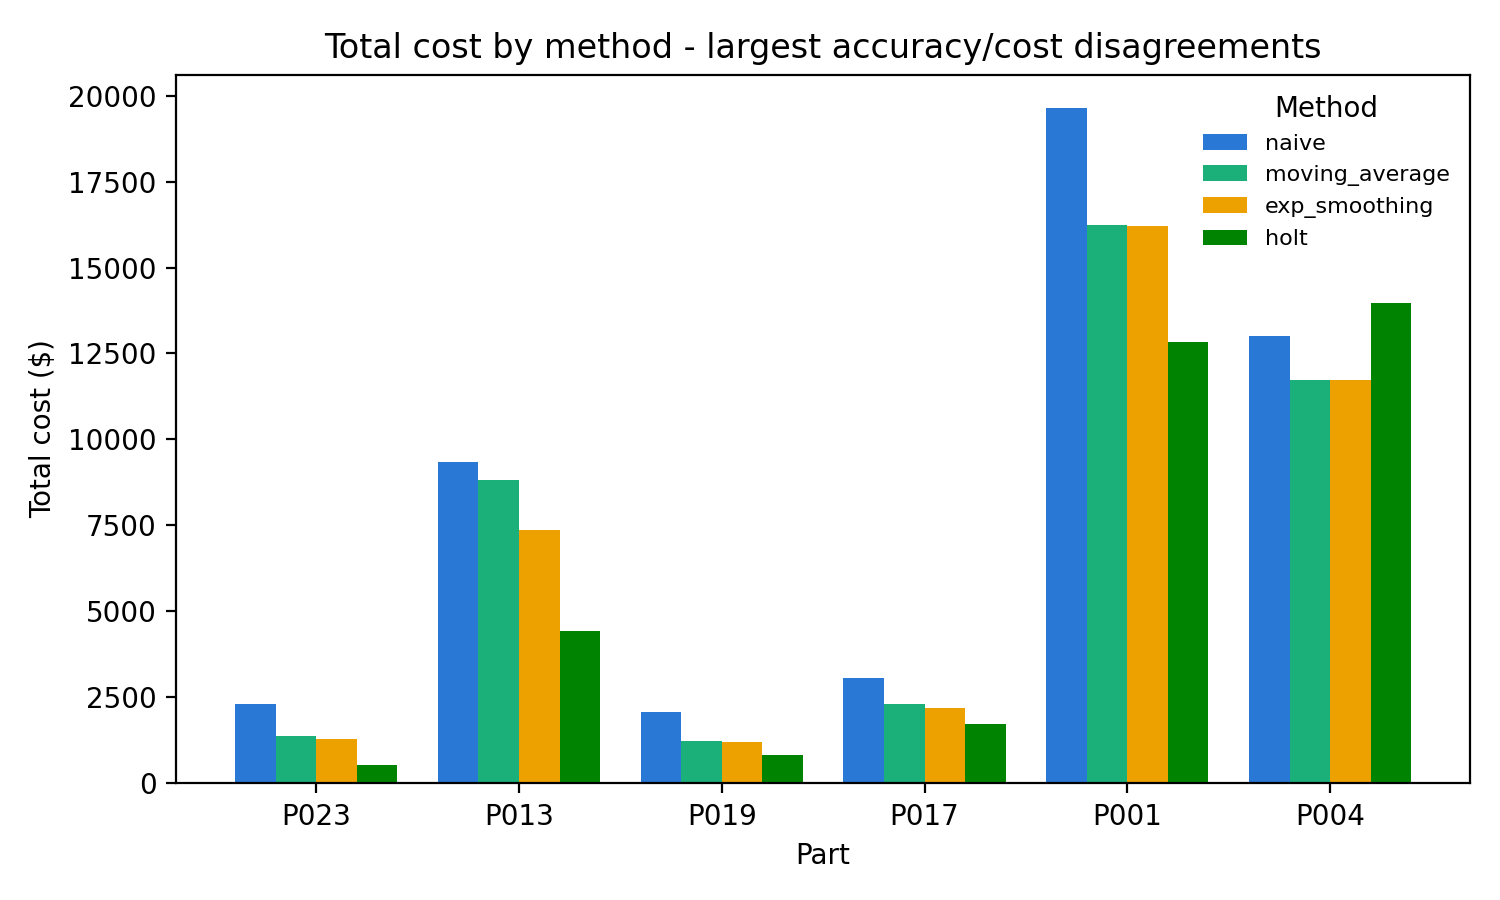
\includegraphics[width=0.85\textwidth]{figures/disagreement.png}
  \caption{Total cost by method for the parts with the largest accuracy/cost disagreement.
  Holt (green) is the cheapest bar for five of six parts shown, but the most expensive for
  P004 -- the same method flips from best to worst choice depending on the part's cost
  structure.}
  \label{fig:disagreement}
\end{figure}

\textbf{Mechanism:} the driver is bias direction combined with cost asymmetry, not raw error
magnitude. Parts P004 and P008 sit in the expensive/high-demand segment
(Figure~\ref{fig:segmentation}), where stockout cost dominates holding cost by roughly 10x --
visible for most parts in Figure~\ref{fig:asymmetry} -- and this asymmetry is the engine of the
entire finding: without it, which direction a method's errors lean would not matter for cost
at all. On the high-stockout-cost parts, Holt's slightly stronger under-forecasting bias is
punished disproportionately by the high per-unit stockout cost, even though its average error
(MAE) was smaller than the alternative method's.

\begin{figure}[h]
  \centering
  \begin{minipage}{0.48\textwidth}
    \centering
    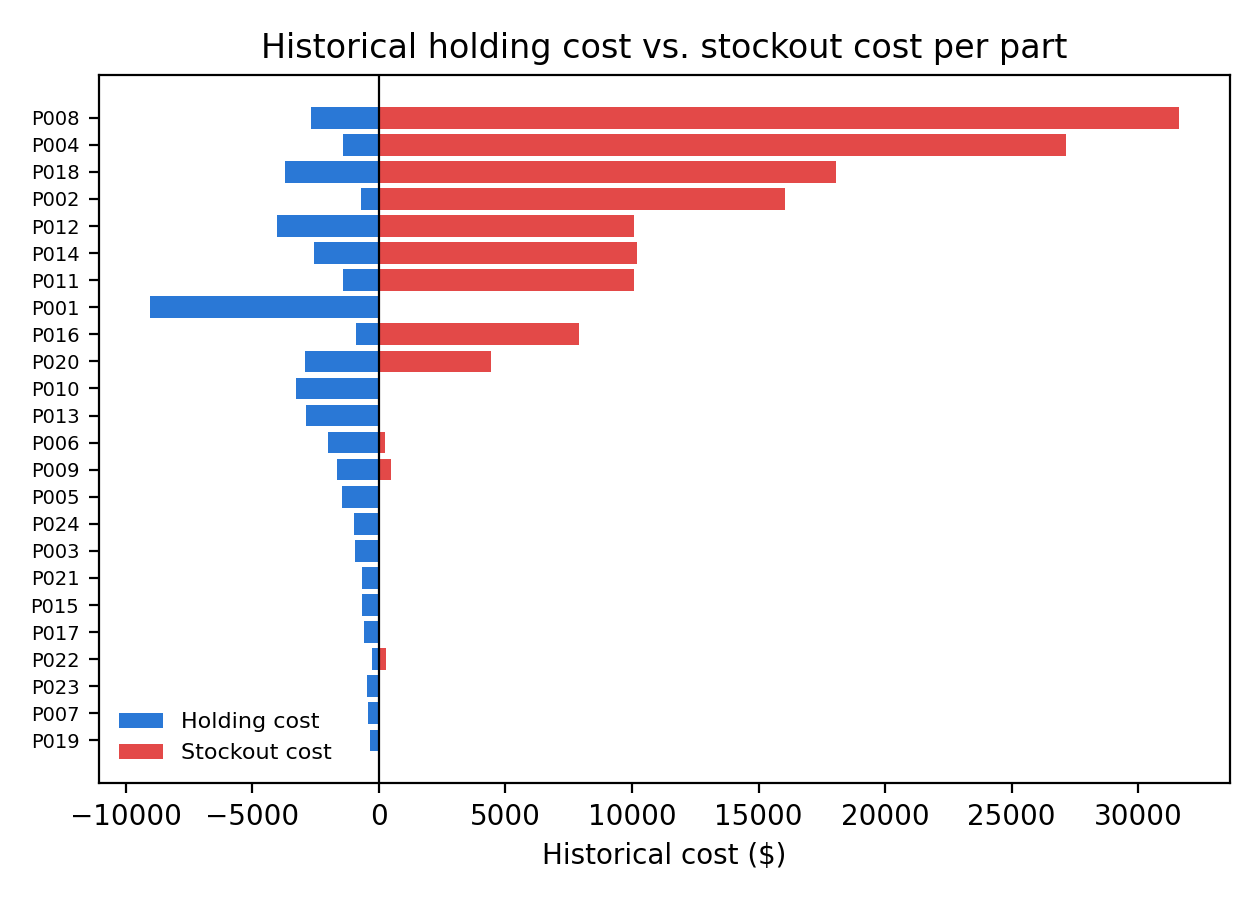
\includegraphics[width=\textwidth]{figures/asymmetry.png}
    \caption{Historical holding cost (blue) vs.\ stockout cost (red) per part. Stockout cost
    dominates for most parts -- the reason bias direction, not error magnitude, drives cost.}
    \label{fig:asymmetry}
  \end{minipage}
  \hfill
  \begin{minipage}{0.48\textwidth}
    \centering
    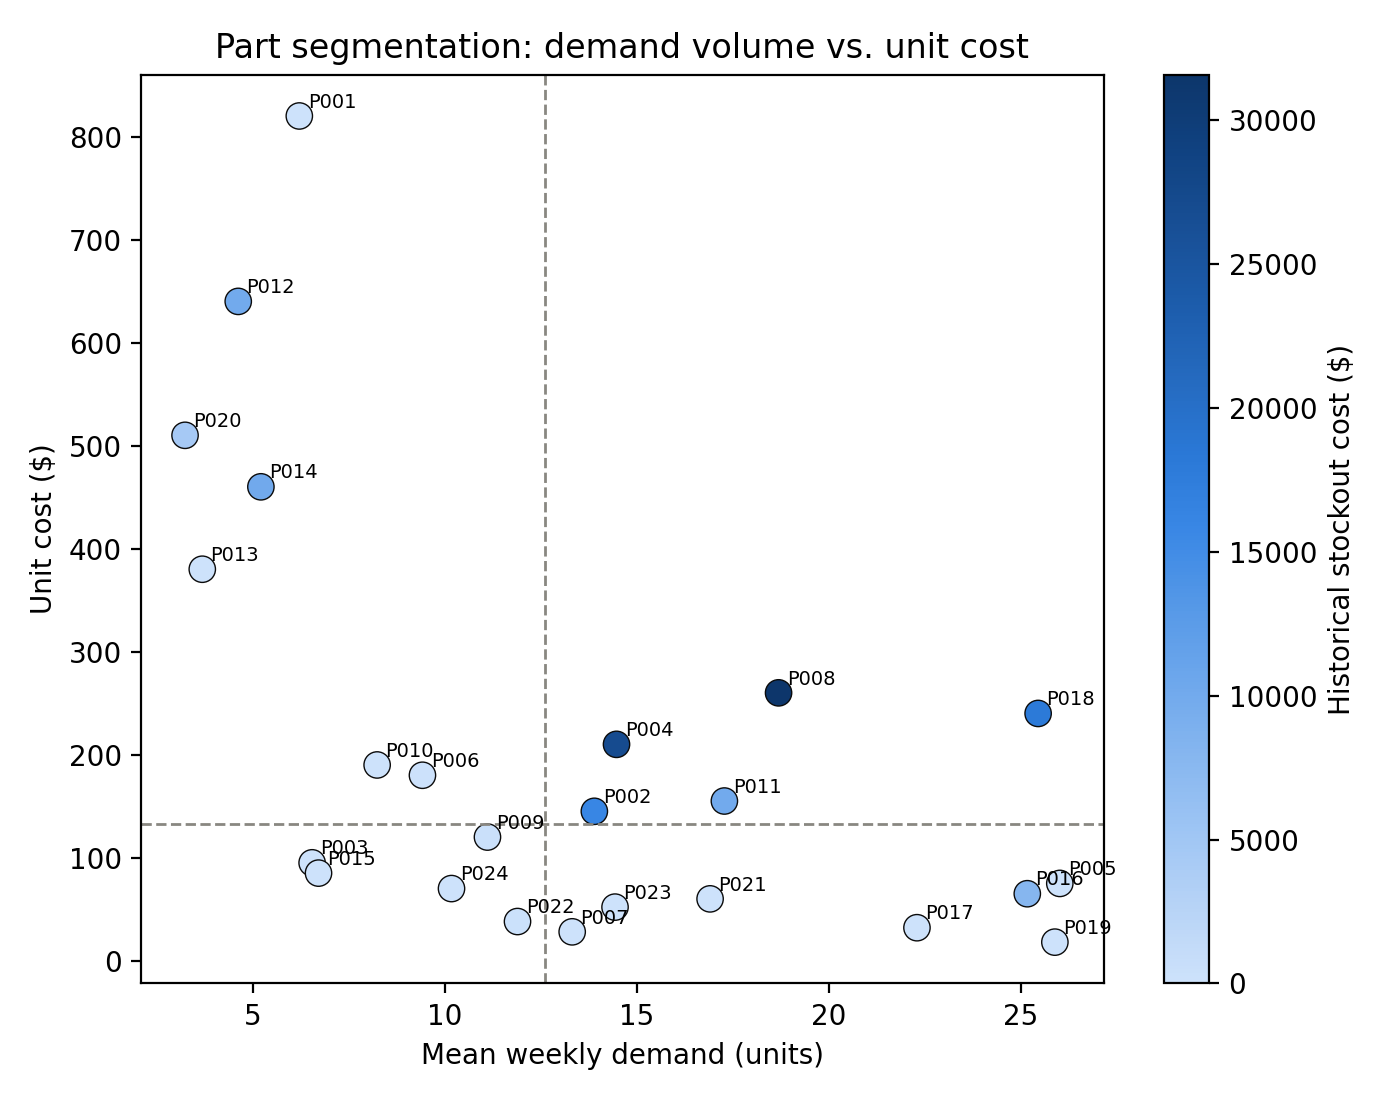
\includegraphics[width=\textwidth]{figures/segmentation.png}
    \caption{Parts segmented by demand volume and unit cost (median split), colored by
    historical stockout cost. The expensive/high-demand quadrant carries the largest exposure.}
    \label{fig:segmentation}
  \end{minipage}
\end{figure}

\textbf{Business recommendations:}
\begin{enumerate}[nosep]
  \item \textbf{Do not select a forecasting method by accuracy alone.} Evaluate cost per part;
  a globally "best" method (Holt, here) can be the worst choice on specific high-stakes parts.
  \item \textbf{15 of 24 parts require immediate reordering} per \texttt{reorder\_recommen-
  dations.csv}, including three (P002, P006, P016) currently at zero stock on hand.
  \item \textbf{P012 is a stockout-risk part to monitor}, despite currently adequate stock --
  it has a 5.1\% historical stockout rate.
  \item \textbf{P001 and P010 are expensive, low-demand parts}: avoid routine over-ordering:
  their risk is cash tied up in slow-moving inventory, not stockouts.
  \item \textbf{Limitations:} Holt's method occasionally failed to fully converge on short
  series (58--77 points); the 95\% service level is a fixed assumption, not individually
  optimized per part; recommended order quantity restores stock only to the reorder point
  rather than a higher order-up-to target, so a part can re-trigger a reorder soon after; and
  the reorder policy has not yet been tested against future (out-of-sample) data.
\end{enumerate}

% ============================================================
\section*{5. Team Member Contributions}

\begin{center}
\begin{tabular}{@{}p{3.2cm}p{10.5cm}@{}}
\toprule
\textbf{Member} & \textbf{Primary responsibilities} \\
\midrule
\textit{Name 1} & \textit{e.g., data audit, merge, derived variables; problem formulation} \\
\textit{Name 2} & \textit{e.g., EDA, demand classification, segmentation, visualization} \\
\textit{Name 3} & \textit{e.g., forecasting methods, walk-forward engine, dual evaluation} \\
\bottomrule
\end{tabular}
\end{center}

\textit{Fill in actual names, roles, and note explicitly if any member did not contribute.
Roles may be shared, but each member's main contribution should remain identifiable, and every
member should be able to answer questions on any part of the project.}

\clearpage
% ============================================================
\section*{Appendix}

\textbf{A.1 Error and cost metrics by method} (averaged across all 24 parts):

\begin{center}
\begin{tabular}{@{}lrrrrrr@{}}
\toprule
\textbf{Method} & \textbf{MSE} & \textbf{RMSE} & \textbf{MAE} & \textbf{MAPE (\%)} & \textbf{Overage \$} & \textbf{Total cost \$} \\
\midrule
Holt            & 17.59 & 3.88 & 3.17 & 33.66 & 33.07 & 5{,}713.59 \\
Exp.\ smoothing & 18.89 & 4.03 & 3.26 & 34.78 & 32.17 & 6{,}598.02 \\
Moving average  & 20.06 & 4.15 & 3.35 & 35.06 & 34.00 & 6{,}786.27 \\
Naive           & 31.57 & 5.23 & 4.19 & 43.50 & 41.82 & 8{,}307.97 \\
\bottomrule
\end{tabular}
\end{center}

\textbf{A.2 Disagreement detail} -- parts where the most-accurate method differs from the
cheapest, sorted by cost premium:

\begin{center}
\begin{tabular}{@{}lllrrr@{}}
\toprule
\textbf{Part} & \textbf{Most accurate} & \textbf{Cheapest} & \textbf{Acc.\ cost \$} & \textbf{Cheap cost \$} & \textbf{Premium (\%)} \\
\midrule
P023 & moving\_average & holt           & 1{,}379.0  & 545.2     & 152.9 \\
P013 & exp\_smoothing  & holt           & 7{,}363.8  & 4{,}446.6 & 65.6  \\
P019 & moving\_average & holt           & 1{,}247.1  & 836.4     & 49.1  \\
P017 & exp\_smoothing  & holt           & 2{,}195.1  & 1{,}739.8 & 26.2  \\
P001 & exp\_smoothing  & holt           & 16{,}205.8 & 12{,}845.3& 26.2  \\
P004 & holt            & exp\_smoothing & 13{,}962.9 & 11{,}734.5& 19.0  \\
P008 & holt            & moving\_average& 8{,}849.3  & 7{,}653.0 & 15.6  \\
P021 & moving\_average & holt           & 3{,}379.7  & 2{,}999.7 & 12.7  \\
P007 & holt            & exp\_smoothing & 1{,}556.2  & 1{,}401.7 & 11.0  \\
P010 & moving\_average & exp\_smoothing & 5{,}009.6  & 4{,}561.0 & 9.8   \\
P005 & holt            & exp\_smoothing & 5{,}555.6  & 5{,}281.0 & 5.2   \\
\bottomrule
\end{tabular}
\end{center}

\textit{Note: P022 is correctly excluded here. An earlier tie-breaking rule (resolving a
2-way accuracy tie by row order rather than by checking whether any tied method was also
cheapest) had misclassified it as disagreeing; the corrected, order-independent rule shows
its tied accurate methods include the cheapest one, i.e.\ it actually agrees.}

\noindent Average premium across all 11 disagreeing parts: \textbf{35.8\%}.

\end{document}
